\documentclass[11pt]{scrartcl}
\usepackage[sexy]{evan}
\usepackage{multirow}
% \usepackage{amsmath}
\usepackage{array}
% \usepackage{program}
% \usepackage{algorithm}
\usepackage{amsmath}
% \usepackage{algpseudocode}
\begin{document}

\title{Geometry}
\author{Arthur Conmy\footnote{Please send any corrections and/or feedback to \url{asc70@cam.ac.uk}.}}
\date{Part IB, Lent Term 2021}

\maketitle
\begin{abstract}
These brief notes are based on lectures given (virtually) by Professor I. Smith in Lent term 2021. 
Many thanks to Artem, Kene, Daniel and David (and more) for many helpful discussions and clarifications.
Credit is also due to Evan Chen for the style file for these notes\footnote{Available here: \url{https://github.com/vEnhance/dotfiles/blob/master/texmf/tex/latex/evan/evan.sty}.}.


I am trying to continually reorder sections, add in more discussions and cover all the course. I hope by the end of the exams this will seem more complete.
\end{abstract}

% \tableofcontents %todo where are the contents

\section{Notation}

I think most notation is used in the course, except perhaps the following

\begin{itemize}
    \item $\subseteq^\circ$: open set in.
    \item $\mapsto$: always read as `maps to'.
\end{itemize}

\section{Geometry from the abstract lens}

This is (mostly!) a pure course, so we build up our object of study from definitions, and then eventually get to prove interesting things about those object (think IA Groups and taking these weird axioms, and following where they take us through a bunch of results). The following definition is the most important and foundational in this course.

\begin{definition}
[Surface]
\label{surface definition}
A \vocab{surface} is a topological space $\Sigma$ such that every $p \in \Sigma$ has a neigbourhood homeomorphic to $\RR^2$.

In this course, we also impose the conditions that $\Sigma$ is Hausdorff and second countable.
\end{definition}

\begin{remark}
Generalising the above to homeomorphism to $\RR^n$ gives rise to a \vocab{manifold}, a more general object.
\end{remark}

\begin{remark}
Forgotten what Hausdorff means again? Never forget again: a topological space $X$ is Hausdorff iff we can `house off' every pair of points: that is to say $\forall p \neq q$, there exist \textit{disjoint} open sets $U, V \subset X$ such that $p \in U$ and $q \in V$.
\end{remark}

(\ref{surface definition}) is a \textit{local} condition on our topological space. We will want to work with more global properties of our surfaces, so we define \vocab{atlases}.

\begin{definition}
An \vocab{atlas} for a surface $\Sigma$ is a set of open sets called \vocab{charts} $\{ U_i \}$ (indexed by some index set $\mathcal{I}$, say), such that 

\begin{equation}
    \bigcup_{i \in \mathcal{I}} U_i = \Sigma.
\end{equation}

Usually, we associate with each $U_i$ a homeomorphism $\phi_i : U_i \rightarrow V_i \subset \RR^2$ and call $(U_i, \phi_i)$ a \vocab{chart}.
\end{definition}

What's the point of this definition? We know that all $p \in \Sigma$ have local ngbds homeomorphic to $\RR^2$, so don't we essentially already have a bunch of open sets that cover our surface? The elegance of atlases is that they allow us to describe surfaces we do not have a clean parametrisation for \textit{with a single atlas}.

\begin{example}
[Single charts do not suffice]

In IA Vector Calculus, we commonly parametrised $S^2$ by

\begin{equation}
    \sigma(u, v) = \begin{pmatrix}\cos u \sin v\\ \sin u \sin v\\ \cos v \end{pmatrix}
\end{equation}

where $u \in U := [0, 2 \pi]$ and $v \in V := [0, \pi]$. But we can't just choose $U \times V$ as our ngbd to all points on $S^2$; to flesh this point out: if we \textit{tried} to make a homeomorphism $\phi : S^2 \rightarrow U \times V$ we would fail, since $v = 0$ (or $\pi$) leads to the $u$ coordinate being arbitrary and injectivity breaking down \footnote{in addition, there are issues with $U$ not being open}.

Atlasses fix this problem in a clean way. For example can just pick $U = (0, 2 \pi)$ and $V = (0, \pi)$, which then only misses out the north and south poles, and half a great circle that joins them. Another open set that's a rotation of $U \times V$ will then allow us to cover all $S^2$ in two charts.
\end{example}

How might we define a global topology with respect to a bunch of possibly very different charts?

\begin{proposition}
[Global Topology on Surfaces]

Suppose we have a countable collection $(U_\alpha, \phi_\alpha)$, where each $U_\alpha$ is a set, and

\begin{equation}
    \phi_\alpha : U_\alpha \rightarrow V_\alpha \subseteq^\circ \RR
\end{equation}

are \emph{bijections} such that $\forall \alpha, \beta$,

\begin{equation}
    \phi_\alpha(U_\alpha \cap U_\beta) \subseteq^\circ V_\alpha.
\end{equation}

Define

\begin{equation}
    \Sigma = \bigcup_\alpha U_\alpha.
\end{equation}

Then 

\begin{itemize}
    \item There is a topology on $\Sigma$ with $U \subseteq \Sigma$ open iff $\forall \alpha$, 
    
    \begin{equation}
        \phi_\alpha(U \cap U_\beta) \subseteq^\circ V_\alpha.
    \end{equation}
\end{itemize}

Suppose that in addition to the above, $\forall \alpha, \beta$, the transition map 

\begin{equation}
    \phi_\beta \phi_\alpha^{-1}
\end{equation}

is a homeomorphism, and that, as a technical condition to enforce the Hausdorff property,

\begin{equation}
    \{ (x,x) : x \in U_\alpha \cap U_\beta \} \subseteq U_\alpha \times U_\beta 
\end{equation}

is closed in $U_\alpha \times U_\beta$, then with this topology, $\Sigma$ is a topological surface.

\begin{proof}
    This is actually a fair amount trickier than it may look at first. The key idea is to use the bijective nature of $\phi_\alpha$.

    For now omitted, left to \ref{daniels notes}.
\end{proof}

% \begin{equation}
% \end{equation}

\label{daniel topology}
\end{proposition}

\subsection{Surfaces in \RR^3}

In the following subsection, we specialise to surfaces that are subspaces of $\RR^3$. Note that note this is not possible for all surfaces; the classic example is the Klein bottle, which self-intersects when we try and embed it into $\RR^3$, and hence (considering the subspace topology on $\RR^3$) at these points of intersection points do not have local neighbourhoods homeomorphic to $\RR^3$.

\begin{definition}
\vocab{Smooth} means infinitely differentiable.
\end{definition}

\begin{definition}
A \vocab{diffeomorphism} is a homeomorphism that is smooth, and has a smooth inverse.
\end{definition}

\begin{definition}
[Transition map]

The \vocab{transition maps} between charts are intuitively defined (from a restricted domain that's a subset of $V_\alpha$, $\tilde{V}$ say)

\begin{equation}
    \phi_\beta \circ \phi_\alpha^{-1} : \tilde{V} \rightarrow V_\beta
\end{equation}

this maps between open sets in $\RR^2$, and has the explicit, suitably restricted domain

\begin{equation}
    \tilde{V} = \phi_\alpha(U_\alpha \cap U_\beta)
\end{equation}

(the notation gets dense when discussing transition maps, but all we're doing is always making sure things are well-defined).
\end{definition}

\begin{definition}
[Smooth Surface]

A smooth surface in $\RR^3$ is a surface $\Sigma$ given as the union of several $U_i$ such that each transition map is a diffeomorphism.
\end{definition}

\begin{remark}
Note that infinite differentiability is a strong condition; we're trying to set things up so we can prove nice things about shapes in space, worrying about wild real analytic pathologies as little as we possibly can.
\end{remark}

To study smooth surfaces in $\RR^3$, actually we can specialise to certain restricted local parametrisations called \textit{allowable} parametrisations:

\begin{theorem}
The following are equivalent:

\begin{itemize}
    \item $\Sigma$ is a smooth surface in $\RR^3$. 
    \item $\Sigma$ is locally the graph of a smooth function over one of the coordinate planes.
    \item $\Sigma$ is locally cut out by the vanishing set of a smooth function with nonzero derivative. That is, $\forall p \in \Sigma$, there is an open $U \in \RR^3$ such that $\Sigma \cap U = f^{-1}(0)$ where $f : U \rightarrow \RR$ is smooth and $Df|_p \neq 0$.
    \item $\Sigma$ is locally the image of an \vocab{allowable} parametrisation, i.e. some $\Sigma : V \rightarrow \Sigma$ where $V \subset \RR^2$ is open and $D \sigma$ has full rank throughout $V$.
\end{itemize}

\begin{proof}
    This is a particularly heavy part of the course, so I'll only discuss the important ideas here.

    Note that the third statement concerns inverting $f$, and the fourth statement involves a full rank statement, which \textit{if} we were working over maps from $\RR^n$ to $\RR^n$. Both of these statements should strongly suggest we should use the Inverse Function Theorem from analysis. However, our maps are those of the form $\RR^m \rightarrow \RR^n$ where $m \neq n$, this is harder. The submersion theorem and the implicit function theorem are the corollaries of the inverse function theorem needed to show these implications.

    % As further motivation
\end{proof}
\end{theorem}

\subsection{Some tools to help us out}

\begin{theorem}
[Inverse Function Theorem]
Let $f:U \rightarrow \RR^n$ be a $C^1$ function on $U$, where $U \subseteq^\circ \RR^n$. Then there are open subsets $V, W \in \RR^n$ so that $f|_V : V \rightarrow W$ is a bijection, and $f\upharpoonright_V^{-1}$ is differentiable with derivative

\begin{equation}
    (Df|_{f^{-1}(x)})^{-1}.
\end{equation}
\begin{proof}
Ultimate result of IB Analysis and Topology.
\end{proof}
\end{theorem}

\begin{remark}
The derivative expression can be memorised since we can write

\begin{equation}
    f(f^{-1}(x)) = x
\end{equation}

and differentiate, using the chain rule.
\end{remark}

To begin working with different dimensions,

\begin{theorem}
[Submersion Theorem]
Let $f : U \rightarrow V$ where $U \in \RR^n$ and $V \in \RR^m$ are open be locally differentiable at $p$ and have surjective derivative. Then there exist coordinate systems (i.e diffeomorphisms with open sets $U'$ and $V'$) such that in these coordinate systems, $f$ is the \textit{submersion}\footnote{(ignore this waffle) the italics here are because I can't resist saying \textit{submersion} as if I'm a death metal singer. Maybe I need to stop listening to Code Orange while revising.}

\begin{equation}
F(x_1, ... , x_n) = (x_1, ... , x_m).    
\end{equation}

\begin{proof}
As with many analysis results, make convenience of life assumptions that $p=0$ and it is the first $n$ columns of $Df$ that are linearly independent. 

Now we basically force ourselves into the equal dimension setting: define

\begin{equation}
    \Phi(x_1, ... , x_n) = (f(x_1, ... , x_n), x_{m+1}, ... , x_n)
\end{equation}

which, when thought about for a while, is a locally differentiable function around 0 with derivative invertible (we can explicitly write out the derivative matrix). So applying inverse function theorem, $\Phi^{-1}$ exists. Now after thinking for a while, in fact 

\begin{equation}
    f \circ \Phi^{-1}
\end{equation}

is exactly the submersion requested.
\end{proof}
\end{theorem}

\begin{theorem}
[Implicit Function Theorem]
If we have the same setup as in the submersion theorem, but $n = n' + m$ and we break vectors in $\RR^n$ into their $n'$-dimensional component $x$ and their $m$-dimensional component $y$, and the last $m$ columns of $Df$ are invertible locally then there exists $g$ such that

\begin{equation}
    f(x,y) = 0 \Longleftrightarrow g(x) = y
\end{equation}

\begin{proof}
We essentially already have the convenience of life assumption, meaning that applying submersion, in some coordinates $f(x,y) = \tilde{f}(y)$, where the form of $\tilde{f}$ depends on $x$. This means that $f(x,y)=0$ is equivalent to $y = g(x)$, i.e given some $x$, locally evaluate the invertible $\tilde{f}$ and check which $y$ vector is the zero vector in the changed coordinates.
\end{proof}

% \begin{equation}
%     f(x,y)
% \end{equation}
\end{theorem}

\begin{remark}
As far as I can tell, we are mostly using these results as tools to do geometry, not as analysis facts in their own right. For that reason, the proofs have been brief, and indeed we are not careful in specifying `smooth' versus `$C^1$' and so forth. From the lecturers errata page:

\begin{quote}
    When dealing with topological surfaces, all maps are continuous. When dealing with smooth surfaces, all
    maps are smooth, even if I sometimes forget to say so explicitly.
\end{quote}

We will later similarly see such lax checking that conditions hold when we use Picard-Lindelof to deduce curve and geodesic existence.

\label{Ivan Wisdom}

\end{remark}

\section{Getting our hands on some $\RR^3$ surfaces}

Continuing to work with smooth surfaces in $\RR^3$, we can now consider how to measure familiar quantities such as length, area, angle given our $\sigma$ parametrization. A central tool is the \textit{first fundamental form} ... 

The first fundamental form gives a notion of dot product (equivalently, a bilinear form) of our parametrisation $\sigma(u,v)$. Specifically, given some allowable $\sigma$, the bilinear form on the tangent plane to $\Sigma$ at $p$ is

\begin{equation}
    \begin{pmatrix} E & F \\ F & G \end{pmatrix} = \begin{pmatrix} \langle \sigma_u,\sigma_u \rangle & \langle \sigma_u,\sigma_v \rangle \\ \langle \sigma_u,\sigma_v \rangle & \langle \sigma_v,\sigma_v \rangle \end{pmatrix}.    
\end{equation}

We more commonly write
% The standard way of writing the first fundamental form is 

\begin{equation}
    E \dd x^2 + 2F \dd x \dd y + G \dd y^2.
\end{equation}

We've seen similar uses of differentials forms (i.e isolated $\dd x$ etc. terms) before in, for example, IA Vector Calculus. Where do they come from?

\subsection{Differential Forms}
%\footnote{Non-examinable}

This section is largely pulled from \cite{napkin}, however hopefully synthesised for an audience who has finished IB Analysis and Topology.

Recall from that course the following results:

\begin{theorem}
[Projecting derivatives]

    Suppose $f : \RR^m \rightarrow \RR^n$ has components $f_i : \RR^m \rightarrow \RR$ for $1 \le i \le n$. The the following are equivalent

    \begin{itemize}
        \item $f$ is differentiable at $p$.
        \item Each $f_i$ is differentiable at $p$,
    \end{itemize}

    \begin{proof}
        Good exercise (I think).
    \end{proof}
\end{theorem}

This is important since it basically means that to study differentiability of functions $f : \RR^m \rightarrow \RR^n$, we can essentially WLOG let $n=1$.

\begin{theorem}
[Computing derivatives in $n$ dimensions.]
    Suppose that $U \subseteq^\circ \RR^m$ and $f : U \rightarrow \RR$ has continuous partial derivatives at $p \in U$. Then $f$ is differentiable at $p$, with derivative
    
    \begin{equation}
        Df(p)(h) = \frac{\partial f}{\partial x_1}h_1 + \cdots + \frac{\partial f}{\partial x_m}h_m.
        \label{Deriv1}
    \end{equation}

    \begin{proof}
        Actually nowhere near as bad as some analyis proofs. Decompose as a telescoping sum

        \begin{align}
        f(x_1 + h_1, \cdots , x_m + h_m) - f(x_1, \cdots , x_m) \\ 
        = f(x_1 + h_1, \cdots , x_m + h_m) - f(x_1 + h_1, \cdots , x_{m-1} + h_{m-1} , x_m) \\
        + f(x_1 + h_1, \cdots , x_{m-1} + h_{m-1}, x_m) - f(x_1 + h_1, \cdots , x_{m-1}, x_m) \\
        + \cdots \\
        + f(x_1 + h_1, x_2, \cdots , x_m) - f(x_1, \cdots , x_m).
        \end{align}

        And now by an `$m$-$\varepsilon$' proof (i.e $m$ applications of the triangle inequality), we use continuity of the first $m-1$ partial derivatives and existence of the $m$th partial derivative to deduce the desired derivative expression.
    \end{proof}
\label{extracting derivatives}
\end{theorem}

We're doing geometry here, so everything is smooth and has nice derivative expressions like above (see (\ref{Ivan Wisdom})).

Note that we can rewrite (\ref{Deriv1}) as 

\begin{equation}
    Df(p)(h) = \left( \frac{\partial f}{\partial x_1} e_1^* + \cdots + \frac{\partial f}{\partial x_m} e_m^* \right)(h)
\end{equation}

where $e_1^* , \cdots , e_m^*$ is the dual basis to $e_1, \cdots , e_m$, since the derivative result is saying exactly the derivative decomposes into this projection onto all the coordinate directions.

This is the motivation for the $\dd f$ and $\dd x$ notation. Specifically, in the case $n=1$, define $\dd x = e_1^*$. Then

\begin{equation}
    \dd f = Df = \frac{\partial f}{\partial x} \dd x
\end{equation}

So for example when $f = \sin x$, $\dd f = \cos x \dd x$ and we give in to the temptation and write $\frac{\dd f}{\dd x} = \cos x$.

What does $\dd x^2$ mean? This is simply the bilinear form that maps a pair of $\RR^2$ vectors to the product of the projection onto the $x$ coordinates. This motivates the notation for the fundamental forms.

\subsection{The Second Fundamental Form}

The second fundamental form is another bilinear form that is motivated by the divergence of $\Sigma$ from its tangent space locally near a point: by Taylor's, for $h, j$ small,

\begin{equation}
\sigma(u+h,v+j) \approx \sigma(u,v) + h \sigma_u + j \sigma_v + 
\frac12 (\sigma_{uu}h^2 + 2\sigma_{uv}hj + \sigma_{vv}j^2)
\end{equation}

to second order. Hence the divergence from the tangent plane $T_p \Sigma$ locally at $p$ is (to second order)

\begin{align}
        [ \sigma(u+h,v+j) - \sigma(u,v) ].n 
        %= \frac12 ( \sigma_{uu}.n h^2 + 2 \sigma_{uv}.n hj + \sigma_{vv}.n j^2 ) \\ 
        = \frac12 \begin{pmatrix}h & j\end{pmatrix} \begin{pmatrix} n.\sigma_{uu} & n.\sigma_{uv} \\ n.\sigma_{uv} & n.\sigma_{vv} \end{pmatrix} \begin{pmatrix} h\\ j \end{pmatrix}
\end{align} % @todo sort out the horrible formatting here maybe add back in extra line

\begin{definition}
    The second fundamental form $\text{II}$ is defined as the bilinear form appearing above;

    \begin{equation}
        \text{II} = \begin{pmatrix} L & M \\ M & N \end{pmatrix} = \begin{pmatrix} n.\sigma_{uu} & n.\sigma_{uv} \\ n.\sigma_{uv} & n.\sigma_{vv} \end{pmatrix}.        
    \end{equation}
\end{definition}

% So we define the second fundamental form as the bilinear form
% \begin{equation}
% \end{equation}

\begin{theorem}
[Alternative characterisation of SFF]

\begin{equation}
    SFF = - (Dn)^T D\sigma
\end{equation}

\begin{proof}
Note that $n . \sigma_u = n . \sigma_v = 0$ so we get this from partially differentiating these with respect to $u$ and $v$.
\end{proof}

\end{theorem}

Since we have an allowable parametrisation everywhere on $\Sigma$, we can define a unit normal

\begin{equation}
    \frac{ \sigma_u \times \sigma_v }{|| \sigma_u \times \sigma_v ||}
\end{equation}

everywhere\footnote{Subscripts generally denote partial differentiation.} on $\Sigma$. We define the \vocab{Gauss map} as exactly this map, $N : \Sigma \rightarrow S^2$. It is an intuitive result that this is independent of paramterisation.

\begin{remark}
Important: keep track of dimensions. The Gauss map is a map from (a subset of) $\RR^3$ to (a subset of) $\RR^3$. In what follows however, we will specialise to two dimensional bilinear forms on the tangent space.
\end{remark}

Now also consider $n$ as the map $U \rightarrow S^2$ (defined locally on charts) such that 

\begin{equation}
    n = N \circ \sigma.
\end{equation}

Now since $n . n = 1$ always, in fact $n_u$ and $n_v$ are perpendicular to $n$, so $Dn|_p$ (as a map) always sends things to the tangent plane at $n(p)$ on $S^2$, which of course coincides with the tangent plane at $p$ on $\Sigma$ (denoted $T_p \Sigma$).

So, having begun with the Gauss map between (subsets of) $\RR^3$, we now have a map between (subsets of) $\RR^2$. In fact, since 

\begin{equation}
    Dn|_p = DN|_{\sigma(p)} \circ D\sigma|_p
\end{equation}

by the chain rule, defining

\begin{definition}

\label{shape definition}

The shape operator $\mathbb{S}$ is the negative derivative of the Gauss map 

\begin{equation}
    \mathbb{S} = - D N|_{\sigma (p)}.
\end{equation}

% The following theorem shows that this makes sense as a linear map $T_p \Sigma \rightarrow T_p \Sigma$.
\end{definition}

Considered as a map from the tangent space (in the $\sigma$ parametrization) at $p$ to itself, we have, in the evaluation of the first fundamental form below $\mathbb{S}v = -DN|_{\sigma (p)} D \sigma|_p v = - Dn|_p v$ so\footnote{I am not entirely happy with my symbol pushing here. To elaborate, I am interpreting $\text{I}(v,w)$ as $(D \sigma v)^T D \sigma w$, i.e $v$ and $w$ contain coordinates (two numbers in $\RR$) that $D\sigma$ turn into the familiar first fundamental form expression.}

\begin{theorem}

\label{shape identity}

\begin{equation}
    \text{I}(\mathbb{S}v,w) = \text{II}(v,w)
\end{equation}

\begin{proof}

Follows immediately from the chain rule and characterisations of $\text{I}$ and $\text{II}$ given:

\begin{equation}
    \text{I} (\mathbb{S}v, w) = - v^T (D \sigma)^T (DN)^T (D \sigma) w = - v^T (Dn)^T D \sigma w = \text{II}(v,w).
\end{equation}

We can now use these tools to build further upon the abstract surface formalisms began earlier.

% Our bilinear forms $\text{I}$ and $\text{II}$ are only defined on 2D subspaces of $\RR^3$, but in fact $\mathbb{S}$ always lies in the tangent space $T_p \Sigma$:

% But indeed since $N$ always maps to the normal 
\end{proof}
\end{theorem}


\begin{definition}
[Riemannian metrics on $\RR^2$ subsets.]

We can define a \vocab{Riemannian metric} on a subset $V \subset \RR^2$ by a smooth map

\begin{equation}
    z \mapsto \begin{pmatrix} E(z) & F(z) \\ F(z) & G(z) \end{pmatrix}
\end{equation}

where the map is to positive definite bilinear forms (since a map to matrices would be too general).
\label{rm1}
\end{definition}

The next definition is nothing surprising

\begin{definition}
[Riemmanian metrics on abstract smooth surfaces]

A \vocab{Riemannian metric} on a surface given as an atlas is a map defined for each such atlas as in (\ref{rm1}) with the following compatibility condition on the transition maps $f_{\alpha \beta} := \phi_\beta \circ \phi_\alpha^{-1}$: we unsurprisingly want the first fundamental forms to agree, which amounts to needing the following to hold, and so pretending for a moment we have embedded surfaces in $\RR^3$ with associated parametrizations $\sigma_\alpha$ and $\sigma_\beta$, we would want

\begin{equation}
    (D\sigma_\alpha)^T D\sigma_\alpha = (D (\sigma_\beta \circ f))^T D(\sigma_\beta \circ f)
\end{equation}

but of course we're being abstract, so actually we expand via the chain rule and insist

\begin{equation}
    \begin{pmatrix} E & F \\ F & G \end{pmatrix}_\alpha = (Df)^T \begin{pmatrix} E & F \\ F & G \end{pmatrix}_\beta Df.
\end{equation}
\end{definition}

\begin{proposition}
[Riemannian metric topology]

Given a Riemannian metric $g$, it induces a topology via the metric

\begin{equation}
    d(p, q) = \inf_\gamma L(\gamma)
\end{equation}

where the infinimum is taken over the set of smooth curves with $\gamma(0)=p$, $\gamma(1)=q$.

Moreover, this topology is equivalent to the natural surface topology (\ref{daniel topology}).

\begin{proof}
% The central idea here is to use the fol

\begin{lemma}
[Coarseness of Topology]
Let $\tau_1$ and $\tau_2$ be topologies on a set $X$. Then $\tau_2$ is at least as fine as $\tau_1$ if $\forall x \in X$, and sets $U \subseteq^\circ X$ containing $x$, there exists $U' \in \tau_2$ with $x \in U' \subseteq U$.

\begin{proof}
Just algorithmically find $U'$ for all $x \in U$ and union these all up to find $U$ in $\tau_2$.
\end{proof}
\end{lemma}

Of course, if two toplogies are as fine as each other, they're the same (`$y \le x \le y \implies x=y$').

So how do we show this? Sketch: the key idea is that whenever we're computing lengths, really we're integrating a bunch of $|\sigma_u|$ and $|\sigma_v|$ terms. So localise, and use compactness to deduce lower and upper bounds on the size of these quantities, which in turn leads to bounds for the Riemannian metric topology.
\end{proof}
\end{proposition}

\subsection{Gaussian Curvature}

With the linear algebraic tools setup, we can now move onto to begin to appreciate that random interlude about pizza from IA Vector Calculus (but still no full proofs).


\begin{definition}
[Gaussian Curvature]

Recall that the the shape operator $\mathbb{S}$ (\ref{shape definition}) can be considered as a linear map from the tangent space $T_p \Sigma$ to itself. Therefore we can make sense of its determinant:  % deriative of the normal map $Dn : U \rightarrow \RR^3$ actually always maps into the tangent plane since really $S^2$ is a 2D surface. Hence we can make sense of $\det n$ since it is mapping between vector spaces of the same dimension.

The Gaussian curvature $\kappa$ of a smooth surface in $\RR^3$ is the quantity defined by 

\begin{equation}
    \kappa(p) = \det (\mathbb{S})_p.
\end{equation}
\end{definition}

In practice, we are really going to compute this a bit differently:

\begin{proposition}

\begin{equation}
    \kappa = \frac{LN - M^2}{EG - F^2}
\end{equation}

\begin{proof}
    Recall from (\ref{shape identity}) that 

    \begin{equation}
        \text{I}(\mathbb{S}v,w) = \text{II}(v,w).
    \end{equation}

    So in fact, $\mathbb{S} \text{I} = \text{II}$ which implies the formula after taking determinants.
\end{proof}
\label{det formula}
\end{proposition}

However, there's another characterisation of Gaussian curvature less tied to particular parametrizations.

\begin{proposition}

Let $(A_n)_{n \ge 1}$ be a sequence of nested open neighbourhoods of $p$ that shrink arbitrarily small\footnote{formally, eventually they all lie in $B(p, \varepsilon)$ for all $\varepsilon > 0$.}. Then 

\begin{equation}
    |\kappa| = \lim_{n \rightarrow \infty} \frac{\text{Area}_{S^2}(N(A_i))}{\text{Area}_\Sigma(A_i)}
\end{equation} 

\begin{proof}
    The key idea here is to calculate areas via cross products. We can do this since to calculate areas from $\sigma$ parametrisations we integrate $\sqrt{EG-F^2}$, and this is precisely $\sigma_u \times \sigma_v$.
    
    So (stare at it) if $\sigma(U_i) = A_i$,

    \begin{equation}
        \text{Area}_\Sigma(A_i) = \int_{U_i} ||\sigma_u \times \sigma_v|| du dv.
    \end{equation}

    To deal with the Gauss map area, note that $n = N \circ \sigma$ is itself a paramterisation of the surrounding region of the unit sphere we need. So apply the same formula, extracting the $u$ and $v$ partial derivatives via the total derivative decomposition (\ref{extracting derivatives}),

    \begin{equation}
        \text{Area}_{S^2}(N(A_i)) = \int_{U_i} ||n_u \times n_v|| du dv = \int_{U_i} ||DN(\sigma_u) \times DN(\sigma_v)|| du dv.
    \end{equation}

    Now note that since everything here is linear (and in particular we're in 2D so even direct expansion will suffice), if $(v_1 v_2)$ is the matrix that sends $e_1$ to $v_1$ and $e_2$ to $v_2$, and $L:\RR^2 \rightarrow \RR^2$ is a linear map, then

    \begin{equation}
        \det(Lv_1 Lv_2) = \det (L) \det(v_1 v_2).
    \end{equation}

    So 

    \begin{equation}
        \text{Area}_{S^2}(N(A_i)) = \int_{U_i} |\kappa(u,v)| ||\sigma_u \times \sigma_v|| du dv %  = \int_{U_i} ||DN(\sigma_u) \times DN(\sigma_v)|| du dv.
    \end{equation}

    Now by continuity, we can factor out $|\kappa|$ and get the result.
\end{proof}
\end{proposition}

\begin{remark}
    We can get the sign of kappa, too, by figuring out whether $A_i$ and $N(A_i)$ are similarly orientated.
\end{remark}

\subsection{A first peek at M{\"o}bius transformations} %and the Riemann sphere}

You probably remember the following from IA Groups:

\begin{definition}
A M{\"o}bius transformation $\mathcal{M}$ is a bijection from $\CC_\infty$ to itself given by 

\begin{equation}
    z \mapsto \frac{az+b}{cz+d}
\end{equation}

where $a,b,c,d \in \CC$ and $ad-bc \neq 0$.
\end{definition}

These turn out to have special significance to \vocab{stereographic projection}:

\begin{definition}
\vocab{Stereographic projection} is the map from the unit sphere $S^2$ to the plane $\mathbb{R}^3 \cap \{ z=0 \}$ given by 

\begin{equation}
    (x,y,z) \mapsto \left( \frac{x}{1-z} , \frac{y}{1-z}, 0 \right)
\end{equation}

which is interpreted as projection from the north pole $N$:

\begin{figure}[h]
\centering
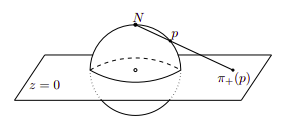
\includegraphics[scale=0.5]{Selection_228.png}
\caption{Stereographic projection (given by the map $\pi_+$).}
\label{fig:stereofig}
\end{figure}
\end{definition}

\begin{exercise}
Check the formula works!
\end{exercise}

\begin{remark}
Where possible, avoid using the formula, and use nice geometric arguments (brevity is great for clarity, and exams!). This isn't always possible, however (see next claim).
\end{remark}

The important link between M{\"o}bius transformations and stereographic projection is the following:

\begin{definition}
The subgroup $\text{PSU}(2) \le \text{PSL}(2,\CC)$ is given by matrices of the form

\begin{equation}
    \begin{pmatrix}
    a & b \\
    -\bar{b} & \bar{a} \\
    \end{pmatrix}
\end{equation}

where $a\bar{a} + b\bar{b} = 1$.
\end{definition}


\begin{proposition}
Rotations of $S^2$ (namely, the action of $\text{SO}(3)$ on it) correspond 1-to-1 with M{\"o}bius transformations (of the plane) in the group $\text{PSU}(2)$ of unitary matrices in $\text{PSL}(2, \CC)$.
\end{proposition}

% \section{Analysis and VP}
\section{Geodesics}

This part is mostly applying our tool of the first fundamental form in the Euler-Lagrange setting.

\begin{proposition}

Lengths of curves are given by

\begin{equation}
L(\gamma) := \int_\gamma ||\gamma'(t)|| \mathrm{d}t = \int_\gamma \sqrt{E\dot{u}^2 + 2F\dot{u}\dot{v} + G\dot{v}^2} \mathrm{d}t.
\end{equation}
\end{proposition}

\begin{exercise}
Show this (hint\footnote{write $||\gamma'(t)|| = \sqrt{\gamma'(t) . \gamma'(t)}$}).
\end{exercise}

We don't actually want to apply Euler-Lagrange to $L(\gamma)$ directly, since the square root is messy and it turns out we can avoid it, and still get equations that tell us when curves are length minimisers.

\begin{definition}
[Energy]

The energy functional is given by

\begin{equation}
    E(\gamma) := \int_\gamma ||\gamma'(t)||^2 \mathrm{d}t
\end{equation}
\end{definition}

\begin{remark}
Unsurprisingly, $L$ is parametrisation independent (exercise ...). However, WARNING: $E$ is not.
\end{remark}

From here, we can apply Euler-Lagrange to study energy minimisers over curves between two points, since $E$ is an expression in the form

\begin{equation}
    \int f(t,u(t),u'(t),v(t),v'(t)) \mathrm{d}t.
\end{equation}

\begin{proposition}
Doing this, we get the fairly gross geodesic equations

\begin{equation}
    \frac{d}{dt}\left( E\dot{u} + F\dot{v} \right) = \frac12 \left( E_u \dot{u}^2 + 2F_u \dot{u}\dot{v} + G_u \dot{v}^2 \right)
\end{equation}

and 

\begin{equation}
    \frac{d}{dt}\left( F\dot{u} + G\dot{v} \right) = \frac12 \left( E_v \dot{u}^2 + 2F_v \dot{u}\dot{v} + G_v \dot{v}^2 \right).
\label{geod 2}
\end{equation}

\end{proposition}

\begin{remark}
As with most Euler-Lagrange things, these need not be committed to memory; the Euler-Lagrange idea of considering small perturbations $f \mapsto \delta f$ (see any VP notes) is quick to rederive even in timed conditions.
\end{remark}

As promised, we now show that studying geodesics, i.e length minimisers, amounts to studying $E$ minimisers:

\begin{proposition}
[Integral Cauchy-Schwarz]

Define an inner product on continuous functions $f : [a, b] \rightarrow \mathbb{R}_{ge 0}$ as follows:

\begin{equation}
    \langle f, g \rangle = \int_a^b f(t) g(t) \mathrm{d}t.
\end{equation}

Then

\begin{equation}
    \langle f, g \rangle^2 \le \langle f,f \rangle \langle g,g \rangle
\end{equation}

With equality iff $f$ and $g$ are scalar multiples.

\begin{proof}
Any Cauchy-Schwarz proof generalises to this infinite dimensional setting with no issues.
\end{proof}
\end{proposition}

Applying C-S with $||\gamma'(t)||$ and the identically $1$ function,

\begin{equation}
    L(\gamma)^2 \le k E(\gamma)
\label{EL Inequality}
\end{equation}

where $k$ is the length of the interval used to parametrise $\gamma$. 
\begin{proposition}
Energy minimisers are length minimisers.

\begin{proof}
Suppose that for contradiction's sake $\gamma$ minimised energy but wasn't a length minimiser. Then pick some $\gamma'$ that was a length minimiser, parametrised with constant speed. Then (\ref{EL Inequality}) gives us that

\begin{equation}
    E(\gamma) > \frac1k L(\gamma)^2 \ge \frac1k L(\gamma')^2 = E(\gamma')
\end{equation}

i.e $\gamma$ isn't in fact an energy minimiser, contradiction.
% so in fact equality must hold, i.e $\gamma$ is parametrised by unit speed 
\end{proof}
\end{proposition}

To avoid using the messy geodesic equations, we might be able to use the following alternative characterisation:

\begin{proposition}
Let $\Sigma$ be a smooth surface in $\RR^3$ and $\gamma : [a, b] \rightarrow \Sigma$ be a smooth curve on $\Sigma$. Then $\gamma$ is a geodesic if and only if the derivative of the tangent vector to $\gamma$ is everywhere normal to $\Sigma$.

\begin{proof}
Exercise! Hint\footnote{There are two geodesic equations, and normal to the tangent plane is equivalent to perpendicular to $\sigma_u$ and $\sigma_v$ ... you guess what you need to do!}.
\end{proof}
\end{proposition}

\subsection{Geodesic normal form}

I assume that the rigour won't be covered in exams (and it is pretty technical analysis anyway), so the following will be handwaved:

\begin{proposition}
[Geodesic existence]

$\forall p \in \Sigma$ embedded in $\RR^3$ and all tangent vectors $v$ at $p$, there's a geodesic $\gamma : [0, \varepsilon) \rightarrow \Sigma$ locally, with $\gamma(0) = p$ and $\gamma'(0) = v$.

\begin{proof}
Working with the gross geodesic equations, this is a question about existence of solutions to differential equations, specifically some of the form

\begin{equation}
\begin{bmatrix}
E & F \\
F & G
\end{bmatrix}
\begin{bmatrix}
u'' \\
v''
\end{bmatrix}
=
...
\end{equation}

Where the RHS is some gross (but smooth!) expression in terms of $u$, $v$, $u'$ and $v'$.

Now the first fundamental form is invertible (wth smooth inverse), so after inverting it we're indeed in the Picard-Lindel{\"o}f setting. Strengthening what we proved in Analysis and Topology, it turns out that this smooth setup means solutions are also smooth (proof omitted). Hand wave over.
\end{proof}
\end{proposition}

Given this existence result, we now can make a coordinate system by travelling along the (locally existent) geodesic $\gamma(v)$ and then constructing for every $\gamma(v)$ a geodesic $\gamma_v$ that is perpendicular to $\gamma$ and is tangent to $\gamma$. This can be thought of as a bunch of orthogonal `offshoot' branches from a common stem.

Here's the picture to have in mind:

\begin{figure}[h]
\centering
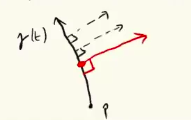
\includegraphics[scale=0.5]{Selection_253.png}
\caption{$\gamma$ is parametrised by $t$, not $v$, but the `offshoot' intuition is shown.}
\label{fig:offshoot}
\end{figure}

\begin{remark}
The curves $u \mapsto \gamma_v(u)$ for fixed $v$ are of course geodesics, but WARNING there's no guarentee that $v \mapsto \gamma_v(u)$ is a geodesic for fixed $u$, except when $u=0$. This is the reason the geodesic normal form doesn't just collapse to something isometric to the plane below!
\end{remark}

% There is at least one detail I am uncertain of here: why $$
% , since then our surface parametrisation would possibly not be continuous (I think). Regardless, if we could, all embedded surfaces in $\RR^3$ would be isometric to the plane, which isn't good!

\begin{proposition}
Embedded surfaces $\Sigma \subseteq \RR^3$ have parametrisations of the form

\begin{equation}
    du^2 + G(u,v)dv^2
\end{equation}

locally.

\begin{proof}
Use (via the handwaving...) the geodesic normal coordinates above: 

\begin{equation}
    \sigma(u,v) = \gamma_v(u).
\end{equation}

% That this is a legitimate parametrisation is mostly straightforward, except why is this injective, i.e: why can't some of the protruding geodesics intersect?

This is an allowable parametrization because at $u=0$, $\sigma_u \perp \sigma_v$ (and both are definitely not vanishing), and hence $D \sigma$ is locally invertible, so by the inverse function theorem locally the parametrisation is invertible, so this is an allowable parametrization indeed ($\sigma$ and $D \sigma$ both injective).

% There's reasonable intuition that this works; thou

$E=1$ follows from the geodesics being parametrised by arc length, but it's not obvious that $F$ is identically zero: we have to use the geodesic equation (\ref{geod 2}) on a curve with $v$ constant, i.e an offshooting geodesic. Then the geodesic equation gives that 

\begin{equation}
    \dot{F} = E_v = 0
\end{equation}

since we saw $E=1$. But on the other hand by the MV chain rule

\begin{equation}
    \dot{F} = F_u \dot{u} + F_v\dot{v} = F_u = 0
\end{equation}

so in fact $F$ is $u$ independent. When $u=0$, $F=0$ so $F \equiv 0$ everywhere.
\end{proof}
\end{proposition}

% @todo write Gaussian curvature part.

An immediate application of this is another, even simpler characterisation of Gaussian curvature

\begin{proposition}

Suppose $\Sigma$ is parametrised by geodesic normal form. Then

\begin{equation}
    \kappa = \frac{\sqrt{G}_{uu}}{\sqrt{G}}
\end{equation}

\begin{proof}
    Just use (\ref{det formula}).
\end{proof}
\end{proposition}

\section{Hyperbolic geometry}

To motivate this section (and it really needs motivation!), we need some heavy machinery:

\begin{definition}
[Triangles on surfaces]

A \vocab{triangle} on a surface is a set of three points on that surface joined pairwise by geodesics.
\end{definition}

\begin{definition}
[Triangulation]

A \vocab{triangulation} of a surface is a graph on the surface where edges are geodesics and where the only faces are triangles\footnote{For the pedantic, more formal definitions can probably be found elsewhere}.
\end{definition}

\begin{definition}
[Euler Characteristic]
The \vocab{Euler characteristic} $\chi(\Sigma)$ of a surface $\Sigma$ is the invariant value

\begin{equation}
    V - E + F
\end{equation}

for a triangulation on that surface.
\end{definition}

The proof of invariance in the plane can be found here: \url{https://en.wikipedia.org/wiki/Euler_characteristic#Proof_of_Euler's_formula}. I don't think that the fact locally surfaces are $\cong \RR^2$ is enough to deduce this fact more generally. See II Algebraic Topology (apparently) for a better definition of $\chi$ as a topological invariant (i.e quantity preserved by homeomorphism).

\begin{theorem}
[Global Gauss-Bonnet]
\label{global gb}

Let $\Sigma$ be an abstract compact smooth surface with abstract Riemannian metric $g$, and Gaussian curvature $\kappa$. Then 

\begin{equation}
    \int_\Sigma \kappa \mathrm{d}A = 2 \pi \chi(\Sigma).
\end{equation}

\begin{proof}
(Black-boxed).
\end{proof}
\end{theorem}

\begin{proposition}
[Donuts!]

Let $\Sigma$ be a surface with \textit{genus}\footnote{for now, work with the informal defintion `number of holes in surface'.} $g$ embedded in $\RR^3$. Then $\Sigma$ has Euler characteristic

\begin{equation}
    \chi(\Sigma) = 2 - 2g.
\end{equation}

\begin{proof}
Sketch: make a triangulation for a torus as a base case, then remove two disk within triangles of two copies of the torus, stitch these together while adding three edges to keep a triangulation and note that the Euler characteristic decreases by 2.
\end{proof}
\end{proposition}

What do we get with all this machinery? Well, suppose we wished to consider metrics on these surfaces that were as symmetrical as possible. Then a natural choice would be to wish for surfaces of constant curvature. By rescaling all the atlases by a factor of $k \neq 0$, namely $\phi \mapsto k \phi$ we would now be assuming $\Sigma$ has curvature $\kappa \in \{ -1, 0, 1 \}$.

We've extensively studied the two non-negative cases here, which correspond to the plane and the sphere). However, (\ref{global gb}) suggests that whenever $g > 1$, we will need to consider the $\kappa = -1$ case.

While we've seen on the example sheet the \textit{tractoid} which has constant curvature $-1$, we will now see that there are much easier (2D!) so-called `models' to work with than that surface.

Eventually, we will actually get to build some $g > 1$ surfaces, and bizarrely this will involve trousers. Stay tuned!

\begin{proposition}
Let $\Sigma = \mathfrak{h}$ the upper half plane model, namely the subset of $\CC$ $\{ z : \text{Im}z > 0 \}$ equipped with the following abstract Riemannian metric:

\begin{equation}
    \frac{\mathrm{d}x^2 + \mathrm{d}y^2}{y^2}.
\end{equation}

Then $\Sigma$ is hyperbolic (i.e has constant curvature -1 throughout 
 $\Sigma$).
 
 \begin{proof}
 Sadly, despite the disk model being probably the most common hyperbolic model we will work with, this comes down a clever trick:
 
 Under the change of coordinates $x = e^{-u} \tanh (v)$ and $y = e^{-u} \text{sech} (v)$ (check that these indeed parametrise in the way we need) we can explicitly calculate $\mathrm{d}x$ and $\mathrm{d}y$ via the multivariable chain rule from IA\footnote{I don't think that formalising this applied math hand-waving with differential forms (i.e $\mathrm{d}x$ etc.) is actually too far out of reach of this course, and it is a nice application of the multivariable calculus developed in Analysis and Topoligy. See \url{https://venhance.github.io/napkin/Napkin.pdf} section XII or even \url{http://pi.math.cornell.edu/~sjamaar/manifolds/manifold.pdf} for a complete exposition. However, I currently do not have a good intuition for why squaring these differential forms is a legitimate manipulation, and this is needed to derive the result.}. Then the metric is
 
 \begin{equation}
     \mathrm{d}u^2 + \cosh^2 (u) \mathrm{d}v^2
 \end{equation}
 
 and hence the Gaussian curvature of $\mathfrak{h}$ is 
 
 \begin{equation}
     - \frac{\sqrt{G}_{uu}}{\sqrt{G}} = -1
 \end{equation}
 
 @todo write the geodesic normal form section to reference the formula.
 
 \end{proof}
 \end{proposition}

Important intuition: if we're given a point to work with in a hyperbolic question, use the disk model with this point as the origin. Alternatively, if we're given a line, use the half-plane model with the line as the (positive) imaginary axis.

\subsection{M{\"o}bius transformations}

At this point in the course, we return to working with inversions and M{\"o}bius transformations, this time in the hyperbolic models. It's easy to get lost in wondering why we're doing all this. To set the record straight

\begin{definition}
In $\mathbb{H}^2$, a \vocab{flag} is a triple consisting of

\begin{itemize}
    \item A (global) geodesic $\gamma$.
    \item A point $p \in \gamma$.
    \item A particular side of $\gamma$.
\end{itemize}
\end{definition}

We care about flags because of the following result, essentially the KEY theorem of the disk models!

\begin{proposition}
Let $\mathcal{F}$ be the set of isometries that act transitively on the set of flags in $\mathbb{H}^2$. Then $\mathcal{F}$ is generated by the M{\"o}bius transformations that preserve the particular model of $\mathbb{H}^2$ that we're working with, and a reflection in a geodesic.
\end{proposition}

\begin{remark}
We only need one particular reflection (e.g $z \mapsto - \bar{z}$, reflection in the imaginary axis\footnote{this works in either model.}) to generate $\mathcal{F}$ due to being able to obtain all such geodesics with MTs.
\end{remark}

\begin{remark}
If we insist such isometries preserve orientation, we in fact only get M{\"o}bius transformations, without the reflections.
\end{remark}

\begin{remark}
In fact we have a uniqueuness statement too: we have a unique hyperbolic isometry that maps a flag to another flag.
\end{remark}

\begin{proof}
One direction here is not too difficult: to show M{\"o}bius transformations are isometries, it is not too difficult to check that their generators are isometries.

The proof that all orientation-preserving isometries are M{\"o}bius transformations is more difficult, and the claims made should be verified! Work in the disk model. Given some orientation-preserving isometry $T$, we can find a M{\"o}bius transformation $M$ such that $M \circ T$ fixes 0 and 1. It's clear that isometries must also preserve geodesics, so in fact $M \circ T$ preserves $\RR \cap D$. In addition, isometries in this model must preserve angles, because if locally an isometry sheared space, then curve lengths would not be preserved\footnote{I would appreciate a clearer reason for this statement!}. So, once again applying geodesic preservation, we have that $i \RR \cap D$ is preserved by $M \circ T$ (it can't be reflected since we're assuming we're in the orientation-preserving case). From this point, the isometry must be the identity since points are determined uniquely by their distance (in hyperbolic, NOT Euclidean metric) to the real and imaginary axis, along with whether they are closest to the positive or negative parts of both of these axes. I made a picture!

\begin{figure}[h]
\centering
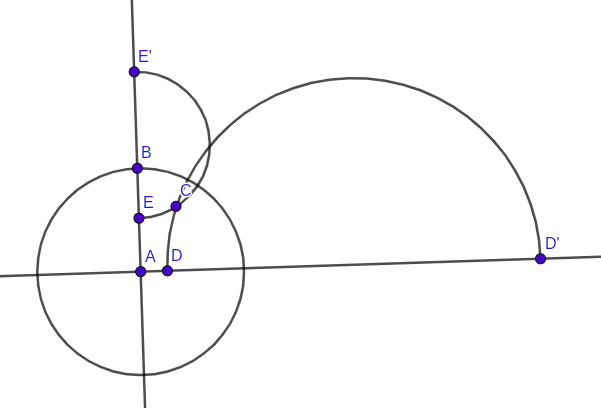
\includegraphics[scale=0.5]{Selection_199.png}
\caption{Given some point $C$ in the disk, the distance of $C$ from the real and imaginary axes are the lengths of the geodesic segments $CE$ and $CD$ shown. This gives rise to the fact that an isometry that fixes $\RR$ and $i\RR$ is in fact the identity.}
\label{fig:firstfig}
\end{figure}

@todo: write orientation preserving section.
\end{proof}

So what actually are the M{\"o}bius transformations that preserve our various models?

\begin{proposition}
In the disk model, the M{\"o}bius transformations that preserve the disk (for the last time, equivalently the orientation preserving isometries!) are those of the form

% \begin{proof}
\begin{equation}
z \mapsto \lambda \frac{z-a}{\bar{a}z-1}
\end{equation}
% \end{proof}

where $|\lambda|=1$ and $|a|<1$.

\begin{proof}
Complex analysis example sheet 1.
\end{proof}
\end{proposition}

\begin{proposition}
In the half-plane model, the relevant M{\"o}bius transformations are those of the form

\begin{equation}
    z \mapsto \frac{az+b}{cz+d}
\end{equation}

where $\begin{bmatrix} a & b \\ c & d\end{bmatrix} \in \text{SL}(2, \RR)$.

\begin{proof}
Sketch: this isn't actually too hard: we need to fix the real line, which quickly yields that all the coefficients need be real, and then we can just isolate the cases $c=0$ and $c \neq 0$. In the former the result falls out quickly, and in the latter case, WLOG $c=1$ so write out

\begin{equation}
    \frac{az+b}{z+d} = \frac{-1}{z+d} + a
\end{equation}

which is the composition of a bunch of two translations and also $z \mapsto - \frac1z$. This final map is an isometry since we have metric

\begin{equation}
    \frac{|\mathrm{d}z|^2}{4 |\text{Im} z|^2}    
\end{equation}

and changing variables to $w = -\frac1z$ preserves this\footnote{Note that again the differential form manipulation should make you a little uneasy...}.
\end{proof}
\end{proposition}

\begin{example}
[The hyperbolic plane is \textit{weird}]

Discuss the example sheet question I think.

This can definitely be skipped for exams.
\end{example}

\begin{proposition}
[Pairs of pants (!)]

Important: the right angles lead to smooth gluing of geodesics.
\end{proposition}

\section{That crazy hard section at the end of the course.}

For the last section of the course, we return to the torus as it arose from the identification space of the square in Analysis and Topology. What happens when we tweak the square?

If we `fix' the torus we're working with, and instead consider exactly what's going on when we change the metric but not the underlying surface

Considering parallelograms with area 1, we can still identify opposite sides and get a pseudo-torus.

Surprisingly, we get \textit{all} flat metrics on the torus this way (no proof).

Somewhat like Gauss-Bonnet, in which we tie a topological invariant (Euler characteristic) to something seemingly unrelated (global curvature) and geometrical, this ties together hyperbolic geometry and a space of metric, which apparently is something studied in higher maths than where we are at now.

\begin{thebibliography}{9}
\bibitem{Napkin}
Evan Chen (2021), \emph{An Infinitely Large Napkin}, \url{https://venhance.github.io/napkin/Napkin.pdf}.

\bibitem{dansnotes}
Daniel Bassett (2021), \emph{IB Geometry}, \url{http://db808.user.srcf.net/Geometry.pdf}.

\bibitem{davidsnotes}
David Bai (2021), \emph{Geometry}, \url{http://zb260.user.srcf.net/notes/IB/geom.pdf}.

% \bibitem{Course Notes}
% Rajen D. Shah (2021), \emph{Mathematics of Machine Learning}, \url{http://www.statslab.cam.ac.uk/~rds37/teaching/machine_learning/notes.pdf}.

% \bibitem{MIT Notes}
% Philippe Rigollet, \emph{18.657: Mathematics of Machine Learning}, \url{https://ocw.mit.edu/courses/mathematics/18-657-mathematics-of-machine-learning-fall-2015/lecture-notes/MIT18_657F15_LecNote.pdf}.

\end{thebibliography}
\end{document}